% -----------------------------------------------
% Template for ISMIR Papers
% 2018 version, based on previous ISMIR templates

% Requirements :
% * 6+n page length maximum
% * 4MB maximum file size
% * Copyright note must appear in the bottom left corner of first page
% * Clearer statement about citing own work in anonymized submission
% (see conference website for additional details)
% -----------------------------------------------

\documentclass{article}
\usepackage{ismir,amsmath,cite,url}
\usepackage{graphicx}
\usepackage{color}
\usepackage{xspace}
\usepackage{siunitx}
\usepackage{caption}
\usepackage{subcaption}
\usepackage{float}


\newcommand{\ml}[1]{\textcolor{blue}{ML : #1}}
\newcommand{\vl}[1]{\textcolor{red}{VL : #1}}

% Title.
% ------
\title{Extended playing techniques: \\
the next milestone in musical instrument recognition}

%\title{Use of metric learning of scattering features improves extended playing techniques recognition}

% Note: Please do NOT use \thanks or a \footnote in any of the author markup

% Three addresses
% --------------
\threeauthors
  {First Author} {Affiliation1 \\ {\tt author1@ismir.edu}}
  {Second Author} {\bf Retain these fake authors in\\\bf submission to preserve the formatting}
  {Third Author} {Affiliation3 \\ {\tt author3@ismir.edu}}

%% To make customize author list in Creative Common license, uncomment and customize the next line
%  \def\authorname{First Author, Second Author, Third Author}

% Four or more addresses
% OR alternative format for large number of co-authors
% ------------
%\multauthor
%{First author$^1$ \hspace{1cm} Second author$^1$ \hspace{1cm} Third author$^2$} { \bfseries{Fourth author$^3$ \hspace{1cm} Fifth author$^2$ \hspace{1cm} Sixth author$^1$}\\
%  $^1$ Department of Computer Science, University , Country\\
%$^2$ International Laboratories, City, Country\\
%$^3$  Company, Address\\
%{\tt\small CorrespondenceAuthor@ismir.edu, PossibleOtherAuthor@ismir.edu}
%}
%\def\authorname{First author, Second author, Third author, Fourth author, Fifth author, Sixth author}


%\sloppy % please retain sloppy command for improved formatting % how about no?

\hyphenation{ma-rim-ba}
\hyphenation{re-cog-ni-tion}
\hyphenation{i-so-la-ted}

\newcommand*{\eg}{e.g.\@\xspace}
\newcommand*{\ie}{i.e.\@\xspace}
\newcommand*{\resp}{resp.\@\xspace}

\sloppy 
\begin{document}

%
\maketitle


%%%%%%%%%%%%%%%%%%%%%%%%%%%%%%%%%%%%%%%%%%%%%%%%%%%%%%%%%%%%%%%%%%%%%%%%%%%%%%%%
%%%%%%%%%%%%%%%%%%%%%%%%%%%%%%%%%% ABSTRACT %%%%%%%%%%%%%%%%%%%%%%%%%%%%%%%%%%%%
\begin{abstract}
The expressive variability in which a musical note can be produced conveys some
essential information to the modeling of orchestration and style. Yet, although
the automatic recognition of a musical instrument from the recording of a
single ``ordinary'' note is now considered a solved problem, the ability of a
computer to precisely identify instrumental playing techniques (IPT) remains largely
underdeveloped, and far below human accuracy. This article provides the first
benchmark of machine listening systems for query-by-example browsing among
among 143 instrumental playing techniques, including the most contemporary, for
16 instruments in the symphonic orchestra, thus amounting to 469 triplets of
instrument, mute, and technique. We identify and discuss three necessary
conditions for significantly outperforming the classical mel-frequency cepstral
coefficients (MFCC) baseline: the inclusion of second-order scattering
coefficients to account for the presence of amplitude modulations ; the
inclusion of long-range temporal dependencies ; and the resort to supervised
metric learning. On the Studio On Line (SOL) dataset, we report a P@5 of $99.7\%$
for instrument recognition (baseline at $92.5\%$) and of $61.0\%$ for instrumental playing technique recognition (baseline at $50.0\%$).
\end{abstract}

%%%%%%%%%%%%%%%%%%%%%%%%%%%%%%%%%%%%%%%%%%%%%%%%%%%%%%%%%%%%%%%%%%%%%%%%%%%%%%%%
%%%%%%%%%%%%%%%%%%%%%%%%%%%%%%%% INTRODUCTION %%%%%%%%%%%%%%%%%%%%%%%%%%%%%%%%%%


\section{Introduction}\label{sec:introduction}

\begin{figure}
        \begin{subfigure}{0.25\textwidth}
                \centering
                \includegraphics[width=\linewidth]{./figs/trumpet_variations/TpC-ord-G4-mf_withaxes.eps}
                \caption{Trumpet note (\emph{ordinario}).}
                \label{fig:TpC-ord-G4-mf_withaxes}
        \end{subfigure}%
        \begin{subfigure}{0.25\textwidth}
                \centering
                \includegraphics[width=\linewidth]{./figs/trumpet_variations/TpC-ord-G3-mf_withaxes.eps}
                \caption{Pitch (G3).}
                \label{fig:TpC-ord-G3-mf_withaxes}
        \end{subfigure}%
        
        \begin{subfigure}{0.25\textwidth}
                \centering
                \includegraphics[width=\linewidth]{./figs/trumpet_variations/TpC-ord-G4-pp_withaxes.eps}
                \caption{Intensity (\emph{pianissimo}).}
                \label{fig:TpC-ord-G4-pp_withaxes}
        \end{subfigure}%
        \begin{subfigure}{0.25\textwidth}
                \centering
                \includegraphics[width=\linewidth]{./figs/trumpet_variations/TpC-brassy-G4-ff_withaxes.eps}
                \caption{Tone quality (brassy).}
                \label{fig:TpC-brassy-G4-mf_withaxes}
        \end{subfigure}%
        
        \begin{subfigure}{0.25\textwidth}
                \centering
                \includegraphics[width=\linewidth]{./figs/trumpet_variations/TpC-sfz-G4-fp_withaxes.eps}
                \caption{Attack (\emph{sfzorzando}).}
                \label{fig:TpC-sfz-G4-fp_withaxes}
        \end{subfigure}%
        \begin{subfigure}{0.25\textwidth}
                \centering
                \includegraphics[width=\linewidth]{./figs/trumpet_variations/TpC-flatt-G4-mf_withaxes.eps}
                \caption{Tonguing (\emph{flatterzunge}).}
                \label{fig:TpC-flatt-G4-mf_withaxes}
        \end{subfigure}
        
       
        \begin{subfigure}[b]{0.25\textwidth}
                \centering
                \includegraphics[width=\linewidth]{./figs/trumpet_variations/TpC-trill-maj2-G4-mf_withaxes.eps}
                \caption{Articulation (\emph{trill}).}
                \label{fig:TpC-trill-maj2-G4-mf_withaxes}
        \end{subfigure}%
        \begin{subfigure}[b]{0.25\textwidth}
                \centering
                \includegraphics[width=\linewidth]{./figs/trumpet_variations/TpC+H-ord-G4-mf_withaxes.eps}
                \caption{Mute (\emph{harmon}).}
                \label{fig:TpC+H-ord-G4-mf_withaxes}
        \end{subfigure}
        
        \begin{subfigure}[b]{0.25\textwidth}
                \centering
                \includegraphics[width=\linewidth]{./figs/trumpet_variations/TpC-voc-harms-C4-mf_withaxes.eps}
                \caption{Phrasing (\emph{d\'{e}tach\'{e}}).}
                \label{fig:TpC+voc-harms-G4-mf_withaxes}
        \end{subfigure}%
        \begin{subfigure}[b]{0.25\textwidth}
                \centering
                \includegraphics[width=\linewidth]{./figs/trumpet_variations/Vn-ord-G4-mf-4c_withaxes.eps}
                \caption{Instrument (violin).}
                \label{fig:Vn-ord-G4-mf-4c}
        \end{subfigure}
        \caption{Ten factors of variations of a musical note.}\label{fig:trumpet-variations}
\end{figure}

The progressive diversification of the timbral palette in Western classical music at the turn of the 20th century is reflected in five concurrent trends:
the addition of new instruments to the symphonic instrumentarium, either by technological inventions (\eg theremin) or importation from non-Western musical cultures (\eg marimba) \cite{sachs2012book};
the creation of novel instrumental associations, as epitomized by \emph{Klangfarbenmelodie} \cite{schoenberg2010book};
the temporary alteration of resonant properties through mutes and other ``preparations'' \cite{dianova2007phd};
a more systematic usage of extended instrumental techniques, such as artificial harmonics, \emph{col legno batutto}, or flutter tonguing \cite{kostka2016book};
and the resort to electronic and digital audio effects \cite{zolzer2011dafx}.
The first of these trends has somewhat stalled: to this day, most Western composers rely on an acoustic instrumentarium that is only marginally different from the one that was available in the Late Romantic period.
Nevertheless, the latter approaches to timbral diversification were massively adopted into post-war contemporary music.
In particular, an increased concern for the concept of musical gesture \cite{godoy2009book} has liberated many unconventional instrumental techniques from their figurativistic connotations, thus making the so-called ``ordinary'' playing style merely one of many compositional options.


Far from being exclusive to erudite music, extended playing techniques are also commonly found in oral tradition; in some cases, they even stand out as a distinctive component of musical style.
Four well-known examples are:
the snap pizzicato (``slap'') of the upright bass in rockabilly,
the growl of the tenor saxophone in rock'n'roll,
the shuffle stroke of the violin (``fiddle'') in Irish folklore,
and the glissando of the clarinet in Klezmer music.
Consequently, the mere knowledge of organology (the instrumental \emph{what?}~of music), as opposed to chironomics (its gestural \emph{how?}), is a rather weak source of information for browsing and recommending music within large audio databases.


Yet, past research in music information retrieval (MIR), and especially machine listening, too rarely acknowledges the benefits of integrating the influence of performer gestures into a coherent taxonomy of musical instrument sounds.
Instead, gestures are either framed as a spurious form of intra-class variability between instruments, without delving into its interdependencies with pitch and intensity;
or, symmetrically, as a probe for the acoustical study of a given instrument, without enough emphasis onto the broader picture of orchestral diversity.

One major cause of this gap in research is the difficulty of collecting and annotating data for contemporary instrumental techniques.
Fortunately, such obstacle has recently been overcome, owing to the creation of databases of instrumental samples in a perspective of spectralist music orchestration \cite{maresz2013cmr}.
In this article, we capitalize on the availability of data to formulate a new line of research in MIR, namely the joint retrieval of organological information (``\emph{what} instrument is being played in this recording?'') and chironomical information (``\emph{how} is the musician producing sound?''), while remaining invariant to other factors of variability, which are deliberately regarded as contextual: where, when, why, by whom, and for whom was the music (in this recording) played.

Figure \ref{fig:TpC-ord-G4-mf_withaxes} shows the constant-$Q$ wavelet transform (CQT) of a trumpet musical note, as played with an ordinary technique.
Unlike most existing publications on instrument classification, which exclusively focus on pitch (Figure \ref{fig:TpC-ord-G3-mf_withaxes}) and intensity (Figure \ref{fig:TpC-ord-G4-pp_withaxes}) as the main factors of intra-class variability, this paper aims at accounting for the presence of instrumental playing techniques (IPT), such as changes in tone quality (Figure \ref{fig:TpC-brassy-G4-mf_withaxes}), attack (Figure \ref{fig:TpC-sfz-G4-fp_withaxes}), tonguing (Figure \ref{fig:TpC-flatt-G4-mf_withaxes}), and articulation (Figure \ref{fig:TpC+H-ord-G4-mf_withaxes}), either as intra-class variability (instrument recognition task) or as inter-class variability (IPT recognition task).
The analysis of playing techniques whose definition necessarily involves more than a single musical event, such as phrasing (Figure \ref{fig:TpC+voc-harms-G4-mf_withaxes}), is beyond the scope of this paper.


Section 2 reviews the existing literature on the topic.
Section 3 derives the task of IPT classification from the definition of both a taxonomy of instruments and a taxonomy of gestures.
Section 4 describes how two topics in machine listening, namely scattering transforms and supervised metric learning, are relevant to address this task.
Section 5 reports the results from an IPT classification benchmark on the Studio On Line (SOL) dataset.


%%%%%%%%%%%%%%%%%%%%%%%%%%%%%%%%%%%%%%%%%%%%%%%%%%%%%%%%%%%%%%%%%%%%%%%%%%%%%%%%
%%%%%%%%%%%%%%%%%%%%%%%%%%%%%%%%  RELATED WORK  %%%%%%%%%%%%%%%%%%%%%%%%%%%%%%%%
\section{Related work}
This section some of the recent MIR literature on the audio analysis of instrumental playing techniques, 
with a focus on the available datasets afferent to each formulation of the problem.

\subsection{Classification of ordinary isolated notes}
The earliest works on musical instrument recognition restricted their scope to individual notes played with an ordinary technique -- with datasets such as MUMS \cite{opolko1989dataset}, MIS, RWC \cite{goto2003ismir}, and Philharmonia -- thus eliminating most factors of intra-class variability due to the performer  \cite{martin1998asa,brown1999jasa,eronen2000icassp,herrera2003jnmr,wieczorkowska2003jiis,kaminskyj2005jiis,benetos2006icassp}.
These works have culminated with the development of a support vector machine (SVM) classifier trained on spectrotemporal receptive fields (STRF), which are idealized computational models of neurophysiological responses in the central auditory system \cite{chi2005jasa}.
Not only did it attain a near-perfect mean accuracy of $98.7\%$ on the RWC dataset, but the confusion matrix of its automated predictions was closely similar to the confusion matrix of human listeners \cite{patil2012plos}.
Therefore, it seems that the supervised classification of musical instruments from recordings of ordinary notes could now be considered a solved problem; we refer to \cite{bhalke2016jiis} for a recent review of the state of the art.

\subsection{Classification of solo recordings}
One straightforward extension of the problem above is the classification of solo phrases, encompassing some variability in melody \cite{krishna2004icassp}, for which the accuracy of STRF models is around $80\%$ \cite{patil2015eurasip}.
Since the Western tradition of solo music is essentially limited to a narrow range of instruments (\eg{} piano, classical guitar, violin) and genres (sonatas, contemporary, free jazz, folk), datasets of solo phrases, such as solosDb \cite{joder2009taslp}, are particularly difficult to design.
This issue is partially mitigated by the recent surge of multitrack datasets, such as MedleyDB \cite{bittner2014ismir}, which has spurred a renewed interest in monophonic instrumental recordings \cite{yip2017ismir}.
In addition, the cross-collection evaluation methodology \cite{livshin2003ismir} allows to prevent the risk of overfitting caused by the relative homogeneity of these small datasets in terms of artists and recording conditions \cite{bogdanov2016ismir}.
To this date, the best classifier of solo recordings is a spiral convolutional network \cite{lostanlen2016ismir} trained on the Medley-solos-DB dataset \cite{lostanlen2018msdb}, \ie{} a cross-collection dataset which aggregates MedleyDB and solosDB following the procedure of \cite{donnelly2015icdmw}.
We refer to \cite{han2017taslp} for a recent review of the state of the art.

\subsection{Multilabel classification in polyphonic mixtures}
Because most publicly released musical recordings are polyphonic, the generic formulation of instrument recognition as a multilabel classification task is the most appropriate for large-scale deployment \cite{martins2007ismir,burred2009icassp}.
However, it suffers from two methodological caveats: first, polyphonic instrumentation is not independent from other attributes of information, such as geographical origin, genre, or key; and secondly, the inter-rater agreement decreases with the number of overlapping sources \cite[chapter 6]{fuhrmann2012phd}.
Such issues are all the more troublesome that there is, to this date, no  annotated dataset of polyphonic mixtures that is diverse enough to be devoid of artist bias.
The Open-MIC initiative, from the newly created Community for Open and Sustainable Music and Information Research (COSMIR), might contribute to mitigating them in the near future \cite{mcfee2016ismir}.

\subsection{Single-instrument playing technique classification}
Lastly, there is a growing interest for studying the role of the performer in musical acoustics, from both perspectives of sound production and sound perception.
Outside of audio signal processing, this topic is connected to other disciplines, such as biomechanics and gestural interfaces \cite{metcalf2014frontiers}.
Nevertheless, the vast majority of the available literature focuses on the range of playing techniques afforded by a single instrument: recent examples include clarinet \cite{loureiro2004ismir}, percussion \cite{tindale2004ismir}, piano \cite{bernays2013smc}, guitar \cite{foulon2013cmmr,su2014ismir,chen2015ismir}, violin \cite{young2008nime}, cello \cite[chapter 6]{chudy2016phd}, and erhu \cite{yang2014fma}.
On the other hand, the few publications which frame timbral similarity in a polyphonic setting do so according to a purely perceptual definition of timbre -- with continuous attributes such as brightness, warmth, dullness, roughness, and so forth \cite{antoine2018isma} -- yet without connecting these attributes to the discrete latent space of playing techniques.
To the best of our knowledge, this paper is the first to formulate the retrieval of expressive parameters of musical timbre at the scale of the symphonic orchestra at large, while expliciting these parameters in terms of sound production (\ie{} through a discrete set of instructions, readily interpretable by the performer) rather than by means of perceptual epithets only.
We refer to \cite{leman2017chapter} for a recent review of the state of the art.


%%%%%%%%%%%%%%%%%%%%%%%%%%%%%%%%%%%%%%%%%%%%%%%%%%%%%%%%%%%%%%%%%%%%%%%%%%%%%%%%
%%%%%%%%%%%%%%%%%%%%%%%%%%%%%%%%%%%  TASKS  %%%%%%%%%%%%%%%%%%%%%%%%%%%%%%%%%%%%
\section{Tasks}
In this section, we distinguish taxonomies of musical instruments from taxonomies of musical gestures.

\subsection{Taxonomies}
The Hornbostel-Sachs taxonomy (H-S) strives to organize the diversity of musical instruments according to their manufactural characteristics only, and is purposefully unaffected by sociohistorical background \cite{montagu2009muzyka}.
Because it offers an unequivocal way of describing any acoustical instrument without any prior knowledge on its afferent playing techniques, it serves as a \emph{lingua franca} in ethnomusicology and museology, especially for ancient or rare instruments which may lack available informants.
The location of the violin in H-S (321.321-71), as depicted in Figure \ref{fig:instrument-dendrogram}, also encompasses the viola and the cello in addition to the violin.
This is because these three instruments, viewed as inert objects share a common morphology, despite differences in posture for the performer: both violin and viola are usually played under the jaw whereas the cello is held between the knees.
Accounting for these differences involves refining H-S with a vernacular taxonomy.
Most instrument taxonomies in music signal processing, including MedleyDB and AudioSet \cite{gemmeke2017icassp}, reach the vernacular level rather than conflating all instruments belonging to the same H-S node.
In some cases, an even finer level of granularity is attained by listing of potential alterations to the instrument -- be them permanent or temporary, at the time scale of more than a single note -- that affect its resonant properties after the end of the conventional manufacturing process, \eg{} mutes and other preparations \cite{dianova2007phd}.
The only example of node in the MedleyDB taxonomy reaching this level is \emph{tack piano} \cite{bittner2014ismir} .

\begin{figure}[t!]
\centering
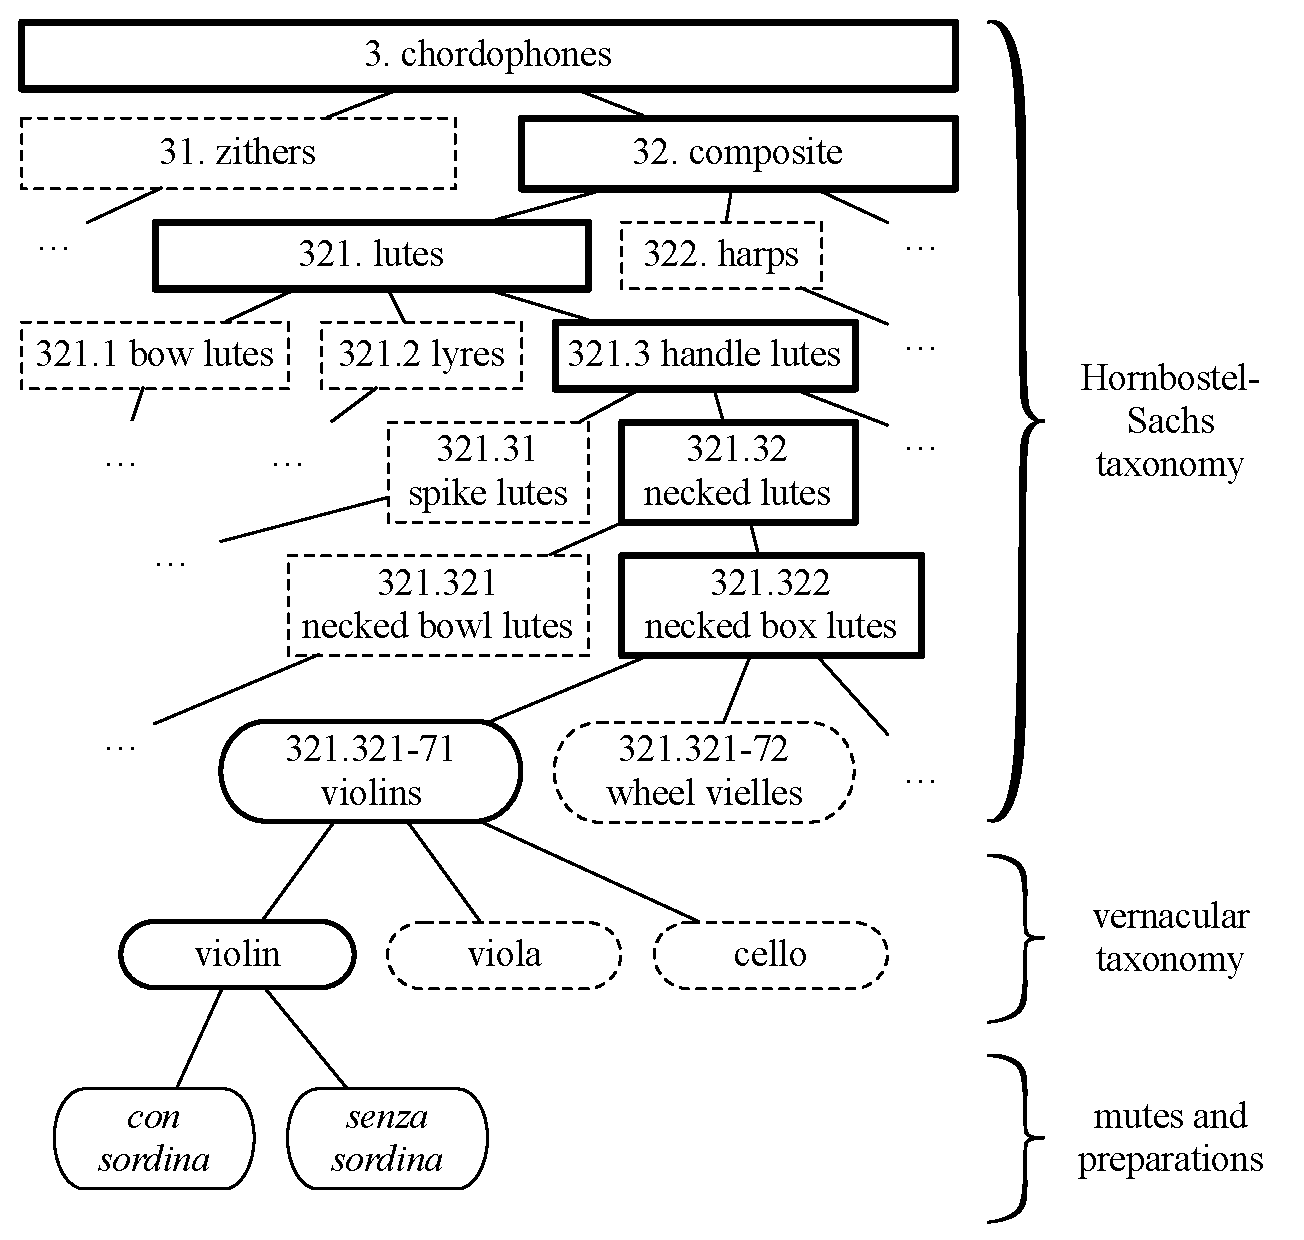
\includegraphics[width=\linewidth]{./figs/dendrograms/instrument-dendrogram.eps}
\caption{Taxonomy of musical instruments.}
\label{fig:instrument-dendrogram}
\end{figure}

Unlike musical instruments, which are approximately amenable to a hierarchical taxonomy of resonating objects, playing techniques result from a complex synchronization between multiple gestures, which may involve both hands and arms, as well as diaphragm, vocal tract, and sometimes the whole body.
As a result, there is no immediate way to interface them with H-S, or any tree-like structure of that sort \cite{kolozali2011ismir}.
Instead, every playing technique is described by a finite collection of categories, each belonging to a different ``namespace''; Figure \ref{fig:technique-dendrogram} illustrates such namespaces in the case of the violin.
It therefore appears that, rather than aiming for a mere increase in granularity with respect to H-S, a coherent research program around extended playing techniques should formulate them as belonging to a meronomy, \ie{} a modular entanglement of part-whole relationships, in the fashion of the Visipedia initiative in computer vision \cite{belongie2015pattern}.
Some music philosophy scholars have begun advocating for supplanting H-S altogether by a modular \cite{magnusson2017jnmr}
However, such considerations are still in large part speculative, and offer no definitive procedure for training, let alone evaluating, information retrieval systems.

\begin{figure}
\centering
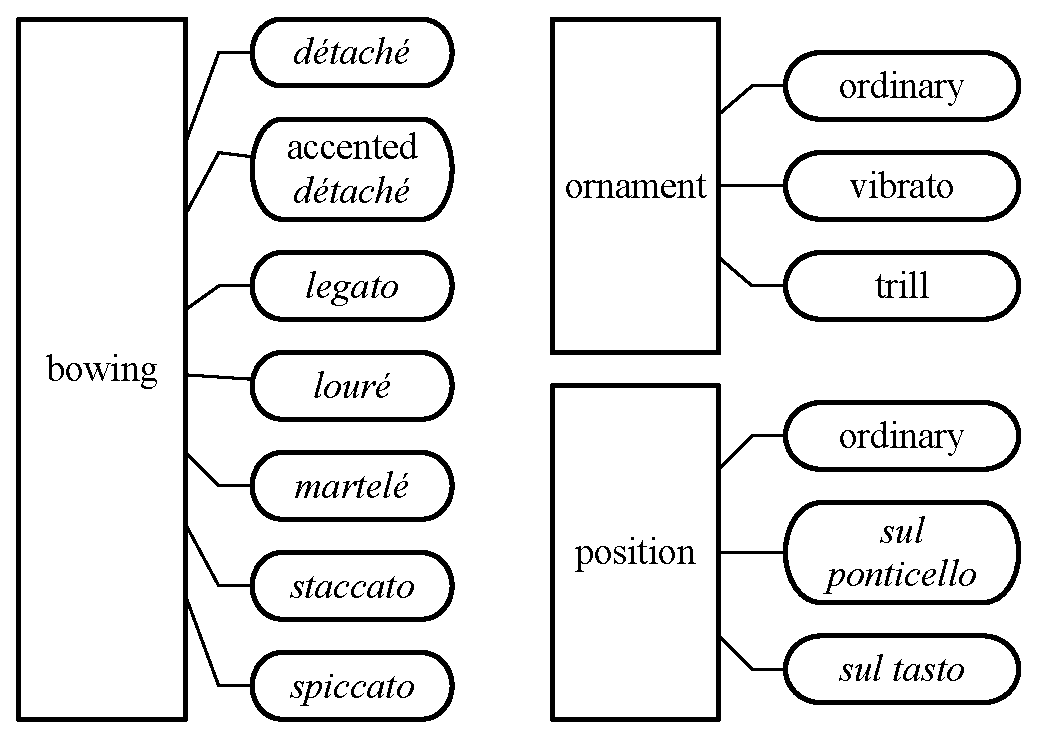
\includegraphics[width=\linewidth]{./figs/dendrograms/technique-dendrogram.eps}
\caption{Namespaces of violin playing techniques.}
\label{fig:technique-dendrogram}
\end{figure}












\subsection{Application setting and evaluation}

\cite{maresz2013cmr}
\cite{lagrange2015jasa}


In this paper, we formulate the instrument / playing techniques recognition problem as a query by example.  We do so as we are \textit{in fine} interested in an application scenario where the user specify a seed sound, be it played by a musical instrument or not, and the system returns several items from the database that have some level of similarity with the seed.

Designing such a system requires the definition of a reference similarity space where the similarity among musical tones is defined perceptually. The aquisition of thus reference is out of the scope of this paper and is left for future work. We thus aim here at numerically validating the processing pipeline considered to implement the query by example system. We would like that such architecture is able to effectively rank items of the database according to 1) the  partition of the musical instruments and 2) the partition of the playing techniques.

To evaluate the performance of the alternative implementations of the query by example system, the precision at rank $k$ is considered. It is computed as the number of relevant items among the $k$ items retrieved by the system divided by $k$. Revelance here is evaluated as the seed and the retrieved item having the same label in the reference partition.

When considering the whole corpus, each item of the database is considered as a seed, and the precision of the system under evaluation is computed for this seed. The precision for this system is the precision averaged over all the seeds. When considering a train /test split corpus, the seeds are taken from the test set and  items of the train corpus similar to this seed are retrieved. The precision for this seed is computed among those retrieved items and the precision for the system under evaluation is the precision averaged over all the items of the test set.

\subsection{Studio On Line (SOL) dataset}


The Studio On Line (SOL) dataset have been recorded at Ircam and is part of the orchestration tools developed in the institute. It is composed of 25444 recordings of single tones played by 16 musical instruments: Accordion, Alto, Bass, Bassoon, Clarinet, Contrabass, Flute, Guitar, Harp, Horn, Oboe, Tenor, Trumpet, Viola, Violin, and Violoncello. The number of recordings per class of instrument is on average 1590 $\pm$936.  Each instrument is played at different nuance and pitch if relevant using 143 different playing technique. The average number of number playing techniques is 178 $\pm$429. The large variance is due to the fact that some playing techniques may be considered for many instruments such as \textit{ordinario}, whereas other are specific to some instruments such as \textit{flatterzunge}. Figure \ref{fig:pt} shows the playing techniques with the higher, lower and median number of recordings.

% YEAR ?
% HISTOGRAM OF PLAYING TECHNIQUES

\begin{figure}[t!]
\centering
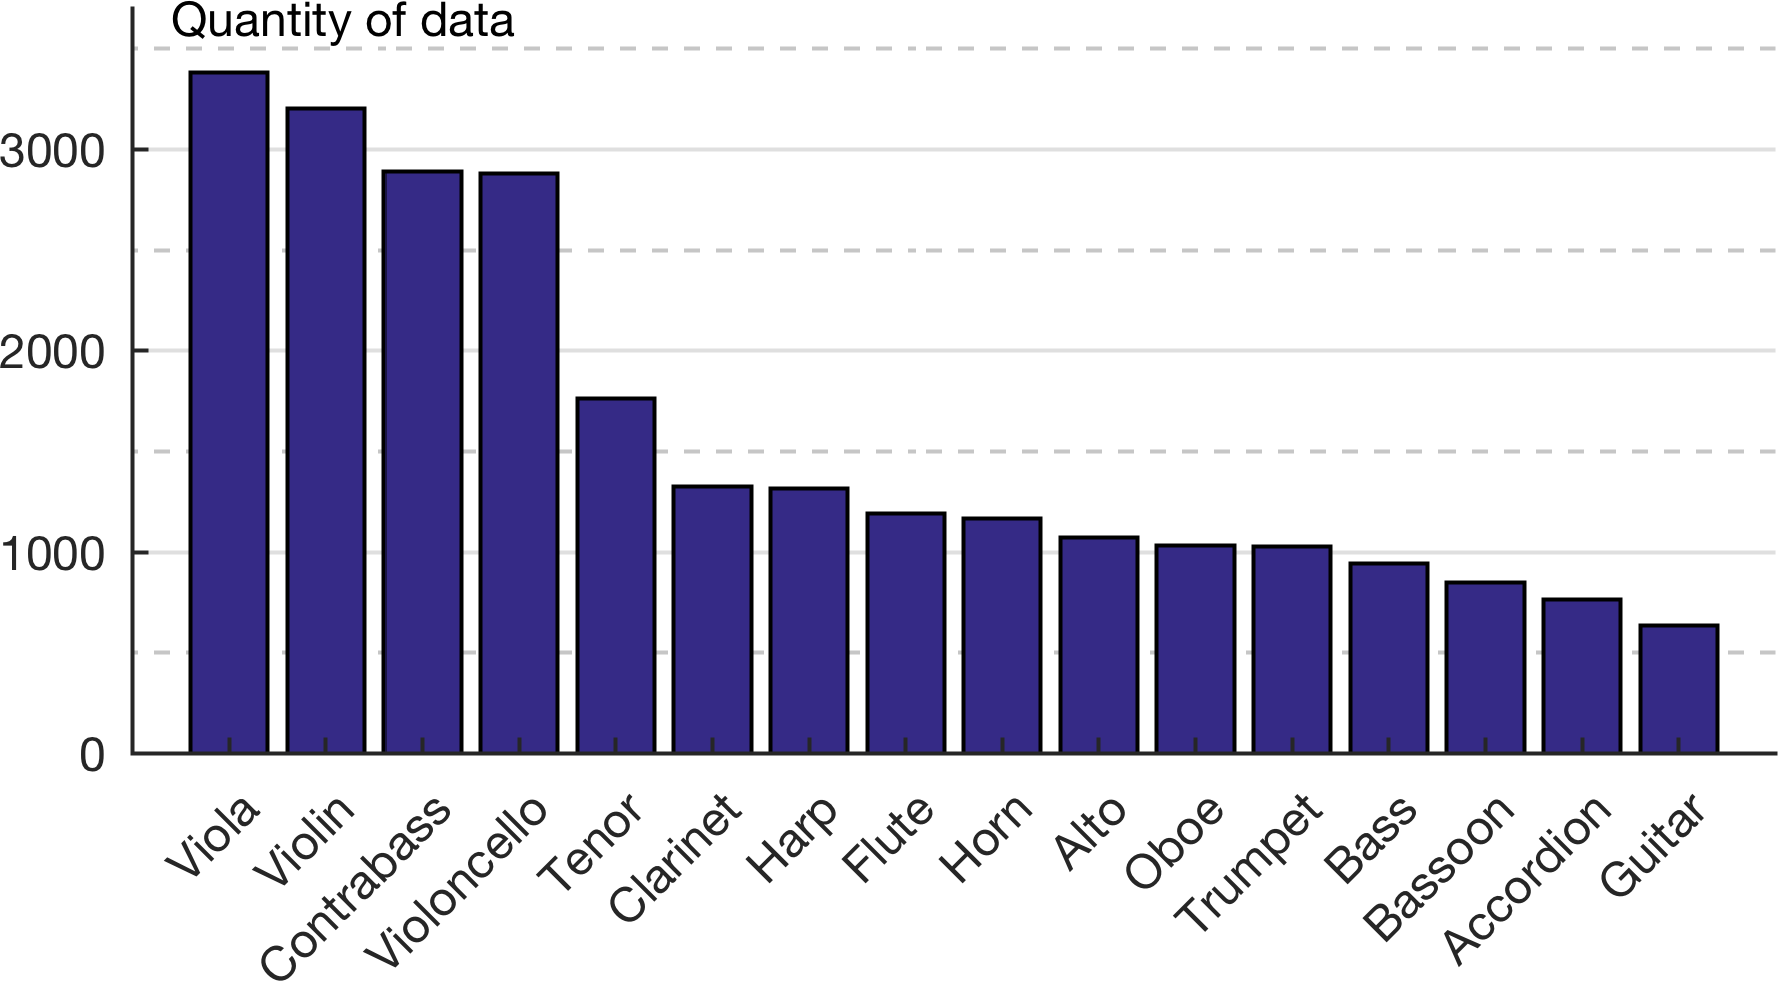
\includegraphics[width=\linewidth]{./figs/histogram/histogram_instruments.png}
\caption{Instruments in the SOL dataset.}
\label{fig:instrument-dendrogram}
\end{figure}


\begin{figure}[h!]
\centering
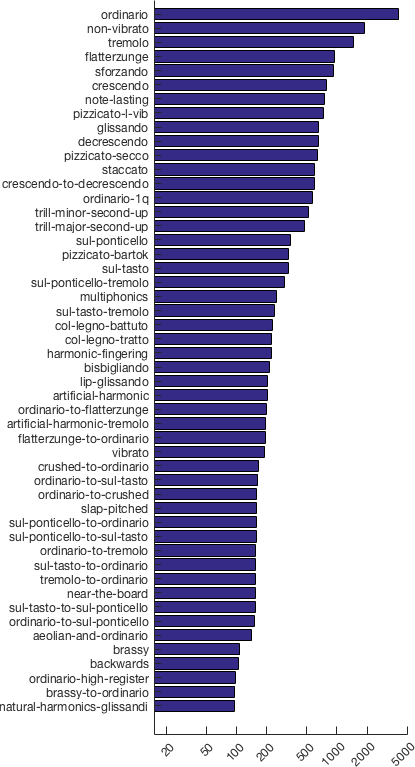
\includegraphics[width=0.96\linewidth]{./figs/histogram/histogram_modes.png}
\caption{Playing techniques in the SOL dataset.}
\label{fig:instrument-dendrogram}
\end{figure}



% Disentangling factors in variability in the production of musical sounds.

% Adopt the Visipedia approach.

% Distinguish what the left hand does from what the right hand does?
% Left hand: vibrato,
% Right hand: tremolo

% Bows and mallets are part of the gesture
% The use of mutes is part of the instrument BUT any gesture while holding the mute (e.g.  trombone) creates a new IPT category that is distinct from ordinary style.

% Out of scope are:
% Variations in articulation: trill, slide. Unlike vibrato, they have a melodic function.
% Variations in: artificial harmonics, subharmonics [ref Mari Kimura],
% Variations in phrasing: arpeggio,
% analog FX:



%%%%%%%%%%%%%%%%%%%%%%%%%%%%%%%%%%  METHODS  %%%%%%%%%%%%%%%%%%%%%%%%%%%%%%%%%%%
\section{Methods}
In this section, we point out the theoretical limitations of mel-frequency cepstral coefficients (MFCC) in the representation of musical sounds comprising with extended instrumental playing techniques (IPT), and describe how both the scattering transform and supervised metric learning may overcome such of these limitations.


\subsection{Scattering transform} % Scattering transform


We refer to \cite{anden2014taslp} for a general introduction to scattering transforms in audio classification, and to \cite{lostanlen2017phd} for a discussion on its application to musical instrument classification in solo recordings.
\cite{anden2012dafx}

\begin{equation}
\widetilde{\mathbf{S}} \boldsymbol{x}_n(\lambda) =
\log \left(
1 + \dfrac{\mathbf{S}\boldsymbol{x}_n(\lambda)}{\varepsilon \times \boldsymbol{\mu}(\lambda)}
\right)
\end{equation}
where $\varepsilon = 10^{-3}$ and $\boldsymbol{\mu}(\lambda)$ is the median value of the scattering coefficient $\mathbf{S}\boldsymbol{x}_n (\lambda)$ for path $\lambda$ across samples $n$ in the training set.

\subsection{Metric learning} % Large-margin nearest neighbors

As shown in the experiments described in Section \ref{sec:exp}, it is helpful to consider a supervised projection of the scattering coefficients in order to select among the large dimensionality of the resulting feature space, which axes are relevant for the task at hand.

May approaches can be considered to achieve such a task \cite{}. One standard approach is the use of the linear discriminant analysis (LDA) that linearly projects ($x \rightarrow L x$) the input data into a features space of $C$-1 dimensions that maximizes the amount of between-class variance
relative to the amount of within-class variance. The linear transformation $L$ is chosen to maximize the ratio of between-class to within-class variance,
subject to the constraint that $L$ defines a projection matrix.


A more flexible approach often taken in metric learning \cite{bellet2013survey} is to optimize a Mahalanobis matrix that linearly projects the input data into another feature space of the same dimensionality. In this case:
\begin{equation}
  M=L^T L
\end{equation}
and the resulting distance cane be expressed as follows:
\begin{equation}
  D_m(x, y) = (x_i-x_j)^T M(x_i-x_j)
\end{equation}
$x_i$ $x_j$ being features vectors. In this study, the large-margin nearest neighbors (LMNN) approach \cite{weinberger2006nips, weinberger2009jmlr} that optimizes the above described performance metric is considered. During the learning process, the following constraints are enforced: : the
k nearest neighbors of any training instance should belong to the
same class of the training instance ( the "pull" constraint) while keeping away instances of other classes (the "push" constraint).

% Write on the Metric Learning to Rank objection ?


%%%%%%%%%%%%%%%%%%%%%%%%%%%%%%%%%%%%%%%%%%%%%%%%%%%%%%%%%%%%%%%%%%%%%%%%%%%%%%%%
%%%%%%%%%%%%%%%%%%%%%%%%%%%% EXPERIMENTAL RESULTS %%%%%%%%%%%%%%%%%%%%%%%%%%%%%%
\section{Experimental results} \label{sec:exp}
In this section, we apply the aforementioned methods to instrument classification and instrumental playing techniques classification in the Studio On Line (SOL) dataset.

\begin{figure}
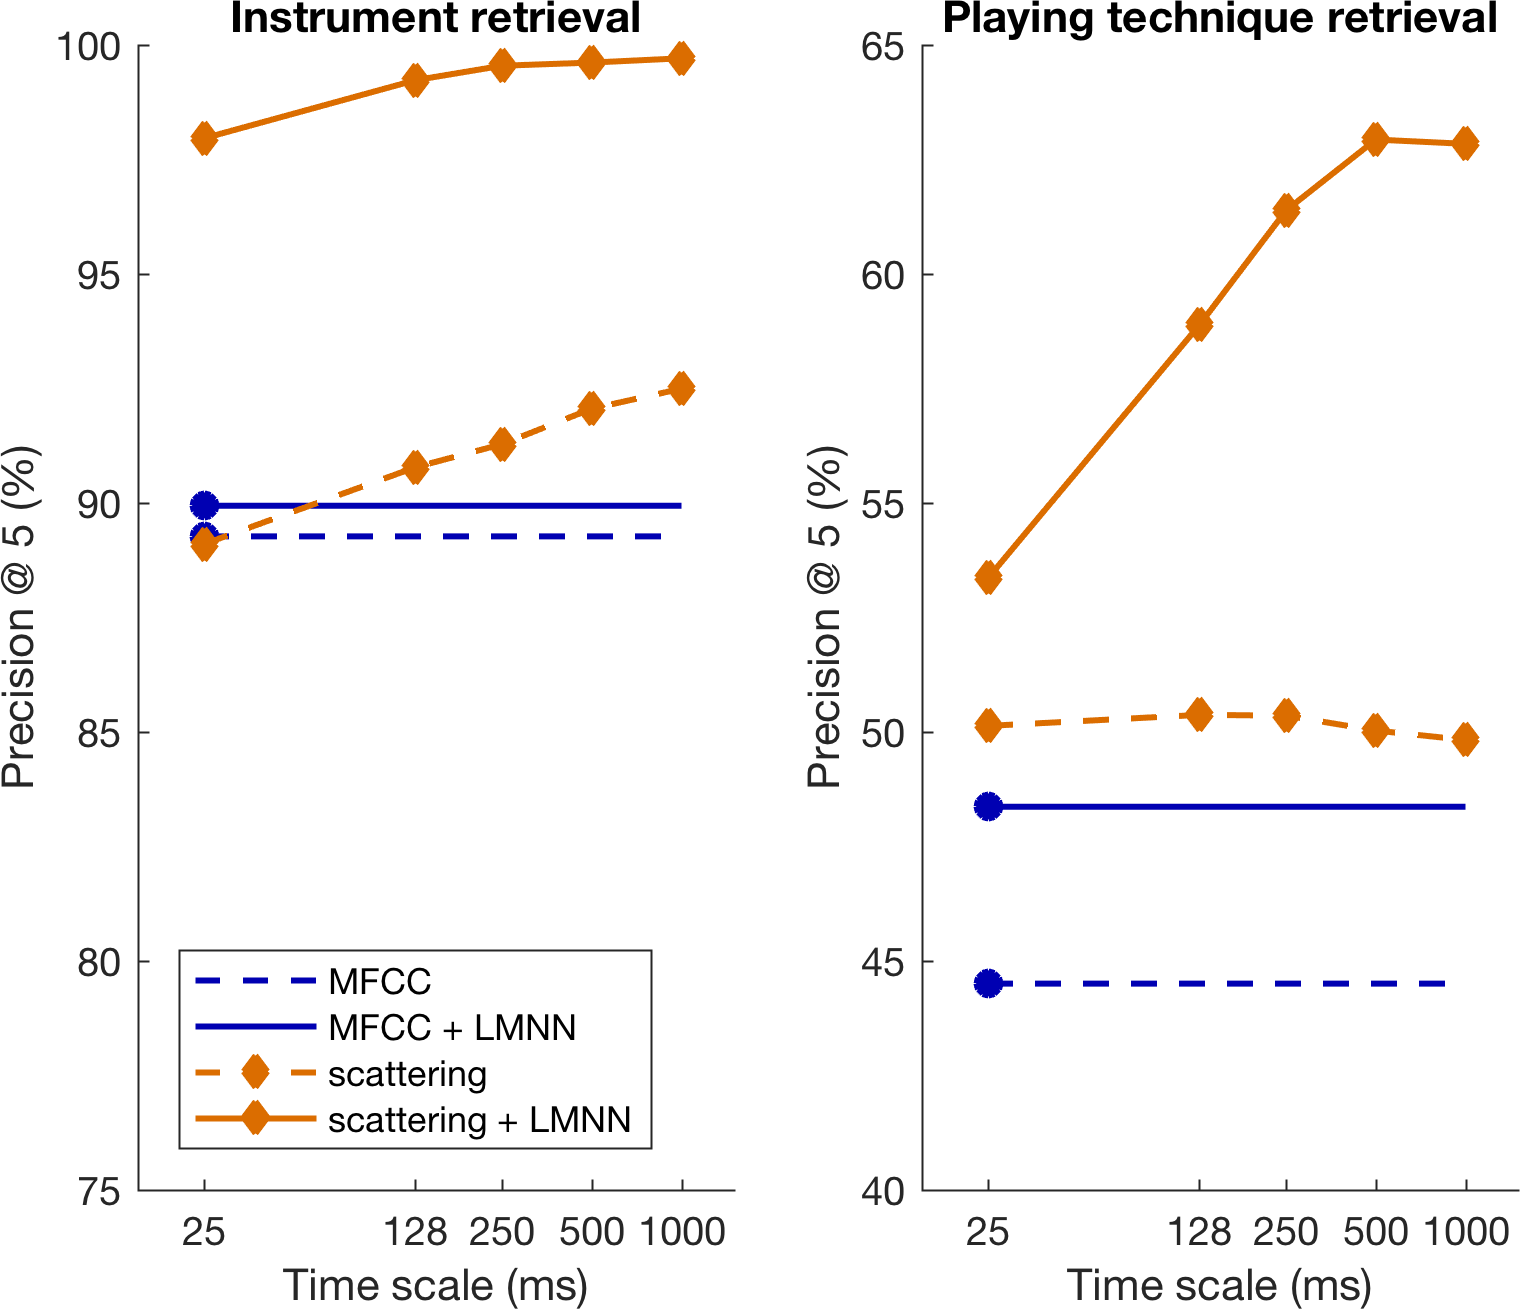
\includegraphics[width=\linewidth,keepaspectratio]{./figs/results/results.png}
\caption{Summary of results on the SOL dataset.}
\label{fig:dataset-statistics}
\end{figure}

\subsection{Evaluation of instrument recognition}

In this section, we report experimental results while considering the musical instruments as the reference. Thus the task aims at grouping together in the feature space, recordings that are played by the same musical instrument regardless of the nuance, pitch and playing technique.

MFCC: $89\%$.
Keeping all $40$ MFCC rather than the lowest $13$ degrades accuracy down to $84\%$.


Scattering: $89\%$.
Disabling median renormalization -- \ie{} setting  $84\%$.
Disabling logarithmic compression altogether: $76\%$.
These results are consistent with \cite{lostanlen2018eurasip}.


\subsection{Evaluation of playing technique recognition}

MFCC: $45\%$. 


\subsection{Pitch-adaptive metric learning}
A well-known rule of thumb in psychoacoustics states that the ``bandwidth for timbre invariance'', \ie{} the musical interval beyond which two notes are judged dissimilar, is of the order of one octave for untrained listeners \cite{handel2001musicperception} and up to $2.5$ octaves for trained listeners \cite{steele2006musicperception}.




%%%%%%%%%%%%%%%%%%%%%%%%%%%%%%%%%%%%%%%%%%%%%%%%%%%%%%%%%%%%%%%%%%%%%%%%%%%%%%%%
%%%%%%%%%%%%%%%%%%%%%%%%%%%%%%%%%  CONCLUSION  %%%%%%%%%%%%%%%%%%%%%%%%%%%%%%%%%
\section{Conclusion}
Every quest for information is also a quest for invariance. [...]
% We have formulated the problem as query-by-example browsing. Another possible formulation would be textual description.

Our main finding is that mel-frequency cepstral coefficients (MFCC), although highly informative for musical instrument recognition in so-called ``ordinary'' notes, fail to discriminate extended instrumental techniques for at least three reasons.
First, they summarize spectral envelope without retaining its amplitude modulations.
Secondly, the frame rate at which they are computed ($T=\SI{25}{\milli\second}$ or so) is short enough to assume local stationarity, but not long enough to encompass all informative local correlations.
Thirdly, the discrete cosine transform (DCT) over mel frequencies does not, contrary to a widespread belief, make them invariant to the frequency transposition of complex sounds.
To address each of these shortcomings, we propose a simple pipeline of three elements: a time scattering transform; an unsupervised renormalization procedure; and a supervised metric learning over frequencies and modulation rates with large-margin nearest neighbors (LMNN).


%\section{Acknowledgments}
% The authors wish to thank Andrew Farnsworth and (?) for fruitful discussions on Visipedia.
% TICEL people.
% Catherine Krocker for helpful suggestions on the title of this article.



% For bibtex users:
\bibliography{lostanlenPlayingTechniques}

\end{document}
